\section{Study Design}
\label{sec:design}

% In this section, we describe the data collection process and 
% the overview of the collected dataset. 
% This section describes our study design, including research questions, data collection, metrics computation, and data description.

\subsection{Research Questions}
\label{sec:rqs}

To identify the characteristics of the visual issue reports, we addressed the following three research questions: focusing on Report (RQ1), Discussion (RQ2), and Fix (RQ3). 
\begin{itemize}
	\item[RQ1:] \textbf{\RQone{}}\\
	Developers often find it difficult to reproduce bugs using the reported information~\citep{DBLP:conf/sigsoft/ChaparroLZMPMBN17}\citep{DBLP:conf/icsm/0001KC20}\citep{zimmermann2010TSE}. 
	On the other hand, as reporters are not always developers, it is not easy to tell what they did and what they encountered~\citep{DBLP:conf/sigsoft/ChaparroBLMMPPN19}. Thus, GitHub developed a feature that can easily provide information with videos and officially announced the feature release on May, 2021~\citep{github-video-blog}. Potter and Faulconer~\citep{POTTER1975} showed that, in general, visual images are a more effective approach for describing what people want to communicate compared with text. 
	We hypothesize that videos or images can reduce the effort for reporting bugs. In this RQ, we measure the number of words in the description of issues as a proxy measure for the effort. 
	\item[RQ2:] \textbf{\RQtwo{}}\\
	Joorabchi \et~\citep{DBLP:conf/msr/JoorabchiMM14} showed that lack of proper communication between reporters and developers often ends up with reports in which the reported bugs are not able to be reproduced. In addition, many studies claim that comments made to a bug contribute to improving bug-fixing activities~\citep{DBLP:conf/icse/GigerPG10}\citep{DBLP:conf/msr/Panjer07}\citep{zhang2012WCRE}.  Visual issue reports might have the potential to attract developers and receive many comments from the developers. In this RQ, we examine the number of comments in the closed issues and the days to receive the first comment.
	% to clarify whether visual can attract developers これは突っ込まれる可能性が高いのでやめとく. 
	\item[RQ3:] \textbf{\RQthree{}}\\
	% We suppose that developers use visualization 
	% in particular issues. 
	% For example, developers may use visualization 
	% to share the way to reproduce bugs. 
	% In this RQ, we clarify the differences 
	% between the issues with and without 
	% visualization. 
	Zimmermann~\et~\citep{zimmermann2010TSE} reported that issue reports occasionally have missing or incorrect steps to reproduce bugs, which delays the entire bug-fixing process~\citep{github-video-blog}. Also, Ohira et al. ~\citep{DBLP:conf/icsm/OhiraHOM12} showed that bug-fixing activities are delayed when the reporter and developer are different persons,  because this situation requires communication between the two.  Visual issues may mitigate this issue by facilitating their communication. In this RQ, we measure the time from reported to closed to evaluate how quickly visual issue reports are resolved, compared with issues without videos or images. 
\end{itemize}

\subsection{Context Selection}
\label{sec:design:context}
To select projects as context for our study, we employed \texttt{GitHub Search}~\citep{msr2021data}. GitHub Search can find repositories satisfying specific criteria. To filter out unpopular, inactive repositories, or repositories that have no issues, we set up the following criteria: the number of stars $\geq$ 10, the number of issue reports $\geq$ 1 and at least one commit was made in 2021.
%\begin{itemize}
%	\item the number of stars $\geq$ 10
%	\item the number of issue reports $\geq$ 1
%	\item at least one commit was made in 2021
% 	\item not include the following tags\\invalid, duplicate, document, question and enhancement
%\end{itemize}
Consequently, the number of the repositories satisfying the criteria was 289,115. From November 2021 to December 2021, we collected 770,655 closed issue reports from 4,173 projects that were randomly selected. 
We collected all the closed issue reports from as many projects as possible in the limited time.  
% if need, please remove the comment out
% However, our studied projects account for only less than 2\% of all the projects. 
% We believe that the selection of repositories is not biased because we randomly selected these repositories. 



% 
\begin{figure*}[t]
\centering
% 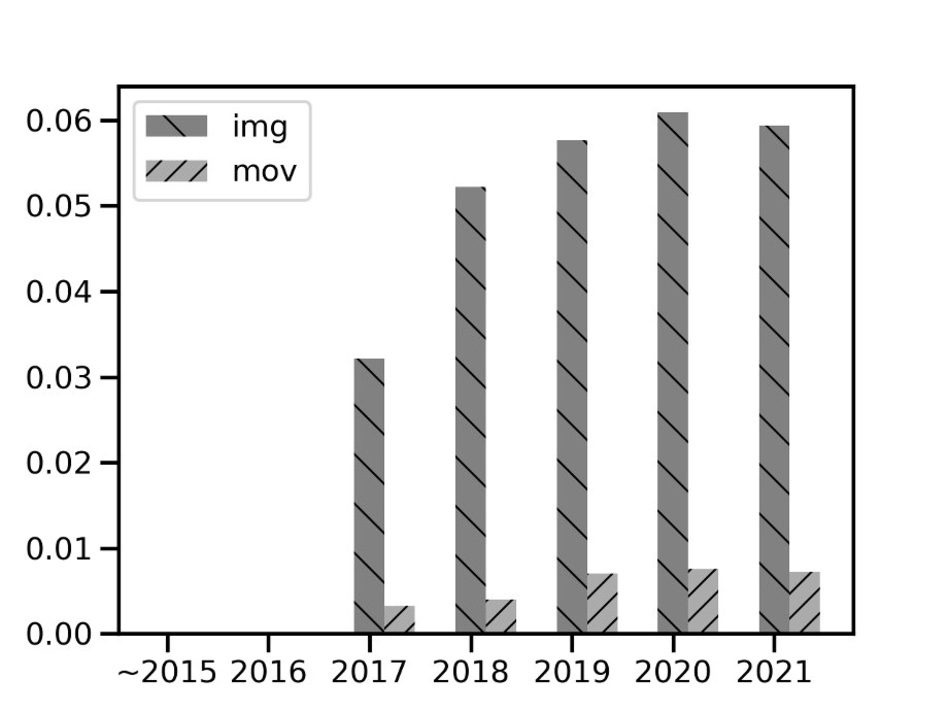
\includegraphics[width=1\linewidth]{./figures/data-category-trend.pdf}
\caption{ 
  An overview of the data collection
  }
\label{fig:data-collection-overview}
\end{figure*}


\subsection{Data Collection}
%\fig{fig:data-collection-overview} shows an overview of the data collection process. 
We first collected closed issue reports with the method \texttt{get\_issue} provided by  \texttt{PyGitHub}\footnote{\url{https://pygithub.readthedocs.io/en/latest/index.html}} that internally execute GitHub API v3.\footnote{\url{https://docs.github.com/en/rest}} In total, we collected 770,655 closed issue reports. 

Next, we collected videos and images attached to the issue reports. While GitHub users can see videos and images on issue pages, the videos and images are stored in different URLs. As the URLs are written in the text description of issue reports, we parsed them with regular expressions and downloaded them. The regular expressions we used are shown as follows:
\begin{quote}
\addtolength\leftmargini{0in}
{\it https://user-images.githubusercontent.com/[a-zA-Z0-9\textbackslash-/]+\textbackslash.[a-zA-Z0-9]+}
\end{quote}
Each downloaded file was determined by its extension to be an image, a video, or neither of these. We used only images and videos. Specifically, ``png'', ``PNG'', ``jpg'', ``JPG'', and ``jpeg'' are treated as images, and  ``gif'', ``GIF'', ``mp4'', ``MP4'', and ``mov'' as videos. 
Consequently, we downloaded 34,553 images and 3,914 videos with the collected URLs. 
%These issues, images, and videos are also included in the dataset (i.e., original dataset) we provide. 

Then, we filtered out inappropriate issue reports for our analysis. As the method \texttt{get\_issue} collects not only issue reports but also pull requests, we excluded pull requests from the original dataset (294,514 issues).  
In addition, unlike Bugzilla~\citep{Bugzilla} or Jira~\citep{JIRA}, GitHub issues do not have resolution statuses (e.g., ``FIXED'', ``DUPLICATED''). 
Instead,  GitHub provides default tags to indicate these resolution statuses. 
We excluded 42,496 issues with tags indicating invalid issues (i.e., ``duplicated'', ``invalid'') or tags indicating non-bug (i.e., ``document'', ``question'', "enhancement"). Also, we removed 25,732 issue reports resolved in too short ($\leq$ 30 seconds) or long periods  ($\geq$ one year) because developers leave bugs for long years without addressing or they report issues after bug-fix. 


\begin{table}[h]
    \begin{center}
    \caption{The number of issues for each category}
    \begin{tabular}{llr}
        \toprule
         & \multicolumn{1}{c}{\textbf{Description}} & \multicolumn{1}{c}{\textbf{\#issues}} \\
        \midrule
        $Img$  & $\#imgs \geq 1$ & 33,079 (4.65\%)\\
        $Mov$  & $\#movs \geq 1$ & 3,819 (0.54\%)\\
        $None$ & Others & 674,793 (94.81\%)\\ 
        \bottomrule
    \end{tabular}
    \label{classify_result}
    \end{center}
\end{table}

\noindent{\bf Dataset summary.} The final dataset contains 226,286 issue reports,  18,760 images, and 1,230 videos. 
These issue reports are classified into three categories based on whether they have either image(s) or video(s). 
\tab{tab:issue-category} shows the number of issue reports for each category. 
Note that issue reports often have both images and videos. 
These issue reports are counted in both $Img$ and $Vid$ categories (only around 0.05\%). 
Thus, the total number of downloaded issue reports (i.e., 226,286) is different from the sum of issues (i.e., 226,405). 
In this paper, we refer to the issue reports in the $Img$ and $Vid$ categories
as \textit{visual issue reports}. 

\begin{figure}[h]
\centering
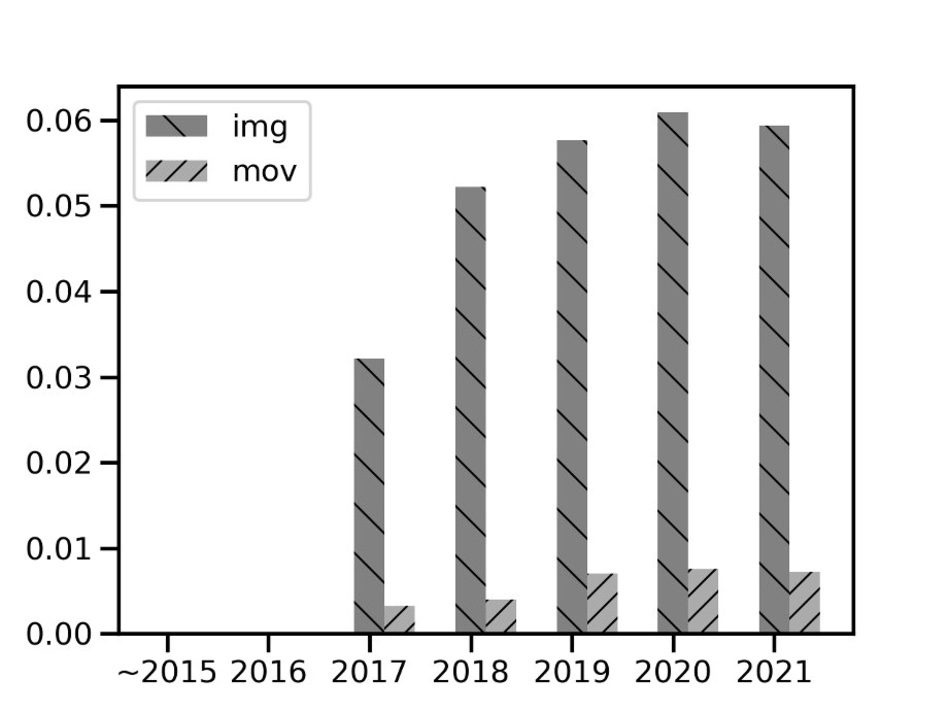
\includegraphics[width=0.6\linewidth]{./figures/data-category-trend.pdf}
\caption{ 
  The proportions of issue reports for each category
  }
\label{fig:data-cat-trend}
\end{figure}
On average, issue reports categorized in $Vid$ have 1.1 videos and issue reports in $Img$ have 1.5 images.  
Out of the collected issues, only 9.09\% of issue reports have images, and 0.54\% have videos. 
While this number seems to be small, looking into the trend shown in \fig{fig:data-cat-trend}, the rate of visual issue reports by year is increasing from 2017 to 2021. 
The ratio of visual issue reports reached to 13\% between 2017 and 2021. 
Also, we found that GitHub officially launched the feature to share videos in May 2021 but developers often had uploaded videos before the beta release of the feature~\citep{github-video-blog-beta}. 
We manually looked into issue reports and then found that GitHub had allowed users to attach GIF files on the descriptions.

% \begin{table*}[h]
    \begin{center}
    \caption{Examples of the retrieved issues with the values of the attributes}
    \begin{tabular}{c c c c c c c} 
      \toprule
      \textbf{IssueCreatedYear} &
      \textbf{ResolutionTime} &
      \textbf{Images} &
      \textbf{Videos} &
      \textbf{Comments} &
      \textbf{FirstCommentTime} &
      \textbf{DescriptionLength} \\
      \midrule
      2020 & 6.99861111 & 0 & 0 & 1 & 6.99861111 & 4430\\
      2020 & 41.9594329 & 1 & 0 & 3 & 17.7784722 & 85\\
      2020 & 43.8850579 & 0 & 0 & 2 & 0.49828704 & 56\\
      2020 & 44.0935532 & 0 & 0 & 4 & 0.91277778 & 33\\
      2020 & 0.14934028 & 0 & 0 & 8 & 0.08077546 & 244\\
      2020 & 59.5670949 & 2 & 0 & 5 & 0.39472222 & 102\\
      2020 & 74.9322569 & 0 & 0 & 0 & -          & 24\\
      \bottomrule
    \end{tabular}
    \label{tab:example-dataset}
    \end{center}
  \end{table*}

% We extract a part of the retrieved issues in \tab{tab:example-dataset}. 
% Each row corresponds to the values of the attributes of an issue. 
%
\begin{table}[t]
    \begin{center}
    \caption{The attributes we collected from the issues}
    \scalebox{0.85}[0.85]{
    \begin{tabular}{ll} 
        \toprule
        \multicolumn{1}{c}{\textbf{Attributes}} & \multicolumn{1}{c}{\textbf{Description}} \\ 
        \midrule
        $IssueResolvedTime$ & The time until the issue is resolved (day) \\
        $FirstCommentTime$ & The time until the first comment (day) \\
        $\#comments$ & The number of comments \\
        $\#chars$ & \masa{im not sure what is this} \\
        $\#imgs$ & \# of attached images when the issue is created \\
        $\#movs$ & \# of attached movies when the issue is created \\
        $\#words$ &  \masa{im not sure what is this} \\
        $IssueCreatedYear$ & The year when the issue is created \\
        \bottomrule
    \end{tabular}
    }
    \label{tab:issue-attr}
    \end{center}
\end{table}


\begin{table}[t]
    \begin{center}
    \caption{The attributes we collected from the issues}
    \scalebox{0.85}[0.85]{
    \begin{tabular}{ll} 
        \toprule
        \multicolumn{1}{c}{\textbf{Attributes}} & \multicolumn{1}{c}{\textbf{Description}} \\ 
        \midrule
        $IssueResolvedTime$ & The time until the issue is resolved (day) \\
        $FirstCommentTime$ & The time until the first comment (day) \\
        $\#comments$ & The number of comments \\
        $\#chars$ & \masa{im not sure what is this} \\
        $\#imgs$ & \# of attached images when the issue is created \\
        $\#movs$ & \# of attached movies when the issue is created \\
        $\#words$ &  \masa{im not sure what is this} \\
        $IssueCreatedYear$ & The year when the issue is created \\
        \bottomrule
    \end{tabular}
    }
    \label{tab:issue-attr}
    \end{center}
\end{table}

\subsection{Analysis}
\noindent{\bf Attributes.} We retrieved attributes from the collected issue reports. \tab{tab:issue-attr} shows six attributes used in this study, which are classified into three dimensions, ``Report'', ``Discussion'', and ``Fix''. 

The attributes in the dimension ``Report'' are extracted from the description of issue reports or attached files when the issue was created. 
In particular, in RQ1, we count the number of words in reports (\ie, $DescriptionLength$) for $Img$, $Vid$, and $None$. 
In addition,  $Images$ and $Videos$ are used to compare the average number of the files attached in reports. 
Note that these attributes are not calculated from either title, not comments (i.e., only descriptions were used). Also, URLs in the descriptions to attach images/videos are not counted as words in $DescriptionLength$.

The dimension ``Discussion'' has two attributes, $Comments$ and $FirstCommentTime$. 
$Comments$ is the number of comments that were made to an issue report. 
We utilize this attribute as a proxy measure of discussion effort. $FirstCommentTime$ is the time difference in days between when the first comment was made and when the issue was reported. 
We use this attribute for measuring developers' interest. 

The dimension ``Fix'' has $ResolutionTime$ which is the time difference in days between when the issue was closed and when the issue was reported. 

\noindent{\bf Method.} For each research question, we measure the median values of the attributes to compare $Img$, $Vid$ and $None$. 
Also we apply a non-parametric test \textit{Steel-Dwass test}~\citep{steel-dwass-test} to evaluate the difference. 
\textit{Steel-Dwass test} performs the multiple comparisons while taking into account the number of comparisons to prevent increases in the family-wise error rate.
The datasets do not follow normal distributions, and do not satisfy homoscedasticity, and therefore are good candidates for analysis using the Steel-Dwass test. 
